%++++++++++++++++++++++++++++++++++++++++
% Don't modify this section unless you know what you're doing!
\documentclass[letterpaper,11pt]{article}
\usepackage{natbib}
\usepackage{float}
\bibliographystyle{unsrtnat}
\usepackage{tabularx} % extra features for tabular environment
\usepackage{amsmath}  % improve math presentation
\usepackage{graphicx} % takes care of graphic including machinery
\usepackage[margin=1in,letterpaper]{geometry} % decreases margins
%\usepackage{cite} % takes care of citations
\usepackage[final]{hyperref} % adds hyper links inside the generated pdf file
\hypersetup{
	colorlinks=true,       % false: boxed links; true: colored links
	linkcolor=blue,        % color of internal links
	citecolor=blue,        % color of links to bibliography
	filecolor=magenta,     % color of file links
	urlcolor=blue         
}
%+++++++++++++++++++++++++++++++++++++++
\begin{document}

\title{Universidade de Aveiro - Estatística Computacional e Simulação \\\textbf{Projeto 2 - Métodos de Monte Carlo em Inferência Estatística e Métodos de Reamostragem}}
\author{Diogo Pedrosa\SUP{(94358)}, Rita Ferrolho\SUP{(88822)}}
\date{Ano Letivo 2021/2022}
\maketitle


\section*{EXERCÍCIO 1} % Exercício 1

Neste exercício, pretende-se calcular os valores corretos dos integrais $I_1$ (1) e $I_2$ (2) pelo Método de Integração de Monte Carlo. Também se pretende determinar os valores estimados para estes integrais, assim como os respetivos erros de Monte Carlo. Por fim, pretende-se comparar os valores estimados com os respetivos valores corretos.

\begin{equation} 
I_1 = \int_0^1 \int_0^1 e^{-\frac{-1}{2}(x^2+y^2)}dxdy
\end{equation}

\begin{equation} 
I_1 = \int_{-2}^{2} \int_{-2}^{2} e^{\frac{1}{2}(x^2+y^2)}dxdy
\end{equation}

\textbf{Passo 1) Sabe-se que:}

\begin{itemize}

\item O Método de Monte Carlo é baseado na aproximação do valor médio dos valores de $g(X_i)$, para $i \in [1,N]$:

\begin{equation} 
E[g(X)] \approx \frac{1}{N} \sum_{i=1}^{N}g(X_i)
\end{equation}

\item Em alternativa, caso $\{X_i\}_{i \in N}$ seja uma sucessão de variáveis i.i.d. de $X$, o valor exato de $E[g(X)]$ também pode ser escrito da seguinte forma:

\begin{equation} 
E[g(X)] =  \lim_{N \to \inf} \frac{1}{N}\sum_{i=1}^{N}g(X_i)
\end{equation}

\item Caso não seja possível resolver analiticamente um integral I pelo Método de Monte Carlo, pode-se calcular o valor desse integral pela Amostragem de Importância, um método que consiste em aproximar um integral segundo a expressão (5), onde \mathcal{A} é o suporte do integral:

\begin{equation} 
I = \int_{\mathcal{A}} f(x)g(x)dx = \int_{\mathcal{A}} g(x)h(x)\frac{f(x)}{h(x)}dx
\end{equation}

\item A estimativa de um integral I, por simulação de Monte Carlo, pode ser obtida com a seguinte expressão genérica (6):

\begin{equation} 
\hat{I} = \frac{1}{N} \sum_{i=1}^{N}g(X_i)\frac{f(X_i)}{h(X_i)}
\end{equation}

\end{itemize}

\textbf{Passo 2) Calcular o valor exato, valor estimado e erro do valor estimado, para o integral $I_1$} \\

Sabe-se teoricamente que o valor do integral $I_1$ não pode ser determinado pelo Método de Monte Carlo. Contudo, $f_{X,Y}=\frac{1}{2\pi}e^{-\frac{1}{2}(x^2+y^2)}$ é a f.d. da variável aleatória normal bivariada $(X,Y)$ quando as marginais $X$ e $Y$ são independentes e normais $N(0,1)$. Resolvendo a integral $I_1$ com o auxílio de $f_{X,Y}$:

\begin{align*}
I_1 & = \int_{0}^{1} \int_{0}^{1}e^{-\frac{1}{2}(x^2+y^2)} dxdy\\
& = \int_{0}^{1} \int_{0}^{1}e^{-\frac{1}{2}x^2} e^{-\frac{1}{2}y^2} dxdy\\
& = \int_{0}^{1}e^{-\frac{1}{2}x^2} dx \int_{0}^{1} \sqrt{2 \pi} \underbrace{ \frac{1}{\sqrt{2\pi}} e^{-\frac{1}{2}y^2}}_{f.d.p \ de \ uma \ N(0,1)} dy\\
& = (\Phi (1) - \Phi(0)) \sqrt{2\pi} \int_{0}^{1} \sqrt{2 \pi} \frac{1}{\sqrt{2\pi} e^{-\frac{1}{2}x^2}} dx\\
& = 2\pi(\Phi(1) - \Phi(0))^2\\
& = 0.7320931
\end{align*}

Aplicando a técnica da Amostragem de Importância, são definidas as seguintes funções como candidatas a funções de importância: 

\begin{equation} 
f_1(x,y) = 1,\ 0 < x,y <1, \ f_2(x,y) = e^{-(x+y)}, \ 0<x,y< \infty
\end{equation}

Note-se que $f_1$ e $f_2$ são as funções densidade de uma distribuição Uniforme e Exponencial bivariada, respetivamente.\\
Utilizou-se uma amostragem de dimensão $N=1000$, valores obtidos a partir das diferentes distribuições consideradas, sendo utilizados no cálculo de $g(x,y)$, tendo sido, posteriormente calculada a média das observações de $g(x,y)$ e que correspondem à aproximação do valor do integral. 
\begin{itemize}
\item Uniforme\\
Neste caso, utilizamos $f_1$. Obtemos então as funções $f_1(x,y)=1\ e \ g(x,y) =e^{-\frac{1}{2}(x^2+y^2)} $
\item Exponencial \\
Neste caso, utilizamos $f_2$. Obtemos então as funções $f_1(x,y)=e^{-(x+y)}\ e \ g(x,y) =\frac{e^{-\frac{1}{2}(x^2+y^2)}}{e^{-(x+y)}} $
\end{itemize}
De seguida apresenta-se uma tabela com os valores das estimativas obtidas para o integral considerando as diferentes f.d.p, bem como os respetivos desvios padrão e erros.

\begin{table}[H]
\begin{center}
\begin{tabular}{|c|c| c| c| c||}
\hline
Função Utilizada & Aproximação & Desvio Padrão & Erro \\
\hline
$f_1$ & 0.7389136 & 0.1510576 & 0.004776862 \\
\hline
$f_2$ & 0.7004373 & 0.921784 & 0.02914937 \\
\hline
\end{tabular}
\caption{aergwerg}
\end{center}
\end{table}

Da análise da tabela conclui-se que a melhor f.d.p a ser usada no método da amostragem de importâncias é a função $f_1$ pois é a que se aproxima mais do valor real 0.7320931. Também apresenta um desvio padrão menor, e o valor erro de Monte Carlo também é menor.\\

\textbf{Passo 3) Calcular o valor exato, valor estimado e erro do valor estimado, para o integral $I_2$} \\

Para o cálculo do integral $I_2$ utilizou-se o Método de Monte Carlo e o Método da Amostragem de Importâncias. Em primeiro lugar, temos de calcular o valor real de $I_2$, para tal foi usado o \textbf{RStudio}, com a função "adaptIntegrate" do pacote "cubature".

\begin{align*}
I_2 & = \int_{-2}^{2} \int_{-2}^{2}e^{\frac{1}{2}(x^2+y^2)} dxdy\\
& = \int_{-2}^{2} \int_{-2}^{2} e^{\frac{1}{2}x^2} e^{\frac{1}{2}y^2}dxdy\\
& = \int_{-2}^{2} \int_{-2}^{2} e^{x^2}e^{-\frac{1}{2}x^2} e^{y^2} e^{-\frac{1}{2}y^2}dxdy\\
& = \int_{-2}^{2} e^{y^2} e^{-\frac{1}{2}y^2}dy \int_{-2}^{2}e^{x^2}e^{-\frac{1}{2}x^2} dx
& = 89.45028
\end{align*}

Como o valor do integral em ordem a $y$ é igual ao integral em ordem a $x$, basta saber o valor de um deles e depois elevar ao quadrado, daí o valor de $I_2$.\\
Para a amostragem de importância foi necessário ajustar $g(x, y)$ ao
intervalo de integração pretendido (de -2 a 2), obtendo uma nova expressão para $g(x,y)$: 

\begin{equation} 
g(x,y) = 4 \times 4 \times e^{\frac{1}{2}(x^2+y^2)}
\end{equation}

Foram gerados 1000 valores de $x$ e $y$, provenientes de uma distribuição uniforme $U(-2,2)$. Em seguida calculou-se a média de $g(x,y )$, o desvio padrão e o erro de Monte Carlo, que serão posteriormente apresentados.

Foi usado também o Método de Monte Carlo, gerando valores de $x$ e $y$, provenientes de uma distribuição normal truncada no intervalo $]-2,2[$, isto é, os valores de $x,y \in ]-2,2[$.\\
Geraram-se $N=1000$ valores de $x$ e $y$ a partir de uma distribuição normal, onde os valores superiores a 2 e inferiores a -2 são rejeitados.

\begin{align*}
I_2 & = \int_{-2}^{2} \int_{-2}^{2}e^{\frac{1}{2}(x^2+y^2)} dxdy\\
& = \int_{-2}^{2} \int_{-2}^{2} e^{(x^2+y^2)} e^{-\frac{1}{2}(x^2+y^2)}dxdy\\
& = \int_{-2}^{2} \int_{-2}^{2} 2\pi \frac{1}{2\pi} e^{(x^2+y^2)} e^{-\frac{1}{2}(x^2+y^2)}dxdy\\
& = \int_{-2}^{2} \int_{-2}^{2}2\pi e^{(x^2+y^2)} \frac{1}{2\pi} e^{-\frac{1}{2}(x^2+y^2)}dxdy\\
& = \int_{-2}^{2} \int_{-2}^{2} g(x,y)   \underbrace{f(x,y)}_{f.d.p \ de \ uma \ distribuição \ normal \ bivariada}  dxdy
\end{align*}

A função $g(x,y)$ equivavle à seguinte expressão:

\begin{equation} 
g(x,y) = 2\pi e^{(x^2+y^2)}
\end{equation}

De seguida calculou-se os valores de $g(x,y)$ para o intervalo considerado, procedendo ao calculo da média de $g(x,y)$.\\
Apresenta-se na tabela em baixo a valor da aproximação obtida , o erro de monte carlo e o desvio obtidos para os dois métodos utilizados.

\begin{center}
\begin{tabular}{|c|c|c|c|} 
\hline
Método Utilizado & Aproximação & Desvio Padrão & Erro de Monte Carlo \\
\hline
Amostragem de Importância  & 86.62921 & 96.36651 & 3.047377 \\
\hline
Método de Monte Carlo & 98.08152 & 339.8993 & 10.74856 \\
\hline
\end{tabular}
\end{center}

Ao analisar a tabela é possível concluir que a Amostragem de Importância obteve melhores resultados que o Método de Monte Carlo. A Amostragem de Importância apresenta um valor de aproximação 98.08152 mais próximo do valor real, 89.45028.  Apresenta ainda um desvio padrão menor, e o valor erro de Monte Carlo também é menor.




\section*{EXERCÍCIO 2}%Exercicio 2
\item Considerou-se a seguinte série temporal,

$$X_t = aX_{t-1} + bX_{t-1}Y_{t-1} + Y_t,$$ 

onde $Y \sim N(0,1)$. Sabe-se que $$S=\frac{\sum_{t=2}^{N}X_tX_{t-1}}{\sum_{t=2}^{N}X_{t-1}^{2}}$$
é o estimador de mínimos quadrados do parâmetro $a$. Suponha-se que os parâmetros do modelo, de dimensão 100, são os seguintes $a=0.4$ e $b=0.1$. 
\begin{enumerate}
\item[2 - a)] Vai-se utilizar o método das réplicas com N = 1000 para se estimar o pârametro $a$, com $N=1000$ réplicas. Para gerar cada réplica utilizou-se o seguinte algoritmo no Rstudio: 
\begin{itemize}
\item Inicializou-se um ciclo para gerar de 1 a 1000 réplicas;
\item Criou-se o vetor $Y \sim N(0,1)$;
\item Inicializou-se o vetor $X$;
\item Definiu-se a semente, $X_1 = Y_1$;
\item Defeniu-se um novo ciclo em que: 
\begin{itemize}
\item Gerou-se os valores de $X_t$, através da fórmula apresentada anteriormente;
\item Determinou-se o estimador $S$ de $a$;
\end{itemize}
\item A estimativa de $a$ guardou-se num \textit{array} $t2$;
\end{itemize} 
Após se calcular todas as réplicas, calculou-se a média de $t2$,pois esta representa uma estimativa do parâmetro $a$.\\ 
No final calculou-se o intervalo de confiança(98\% de confiança), a estimativa do viés do parâmetro, o desvio padrão do estimador, o valor do erro quadrático médio do estimador(EQM) e realizou-se um box-plot do viés amostral.

Para se determinar o intervalo de confiança a $98\%$, com $\alpha = 2\%$, tem-se que $$L_{inf} = \bar{S} - Z_{1-\frac{\alpha}{2}} \frac{S_N}{\sqrt{N}}$$
$$L_{sup} = \bar{S} + Z_{1-\frac{\alpha}{2}} \frac{S_N}{\sqrt{N}}$$
Onde, $S_{N}^2$ é a variância empírica associada à amostra $(S^{(1)},S^{(2)}, \dots ,S^{(N)})$ e $Z_{1-\frac{\alpha}{2}}$ é o quantil de probabilidade $1-\frac{\alpha}{2}$ de uma $N(0,1)$.
Abaixo encontra-se os resultados obtidos do desvio padrão, erro quadrático médio, o intervalo de confiança e o viés numa tabela e também se encontra o o boxplot da amostra dos enviesamentos.
\begin{table}[H]
\begin{center}
\begin{tabular}{|c| c|} 
\hline
Valor real de $a$ & 0.4 \\
\hline
Estimador de $a$ & 0.4123643 \\ 
\hline
$\hat{Vies}$ & 0.0123643 \\
\hline
$\hat{\sigma^2}$ & 0.100879\\
\hline
EQM &  0.02279214 \\
\hline
$IC_{98\%}$ & ]0.4058127; 0.4189159[ \\
\hline
\end{tabular}
\caption{Resultados método das réplicas}
\end{center}
\end{table}

\begin{figure}[h]
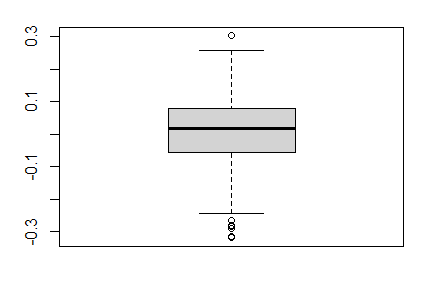
\includegraphics[width=0.5\textwidth]{Box_Plot.png}
\centering
\caption{Boxplot da amostra dos enviesamentos}
\end{figure}
Com a análise do \textit{boxplot}, pode-se observar que a distância inter-quartil é relativamente pequena, o que pode indicar que não existe muita variabilidade de $t2$, isto é, os valores de $t2$ estão muito próximos do valor real de $a$. Observando o valor do desvio padrão pode se corroborar isso, visto que tem um valor reduzido de 0.100879 \\
Consegue-se observar também a presença de outliers no boxplot oq ue pode indicar que em certas réplicas o valor do enviesamento foi superior ao valor originar \\
Relativamente ao intervalo de confiança, pode-se observar que $a$ não pertence ao intervalo, no entanto a amplitude do intervalo é reduzida.\\
Para concluir, fazendo uma suma de tudo pode-se afirmar que o métodos das réplicas produziu um bom estimador de $a$.
\item[2 - b)] Para esta alinea, pretende-se encontrar outra estimativa de $a$, mas aplicando métodos de reamostragem.
Tem-se os seguintes métodos de reamostragem:
\begin{itemize}
\item Método de Bootstrap -  é uma classe de métodos de Monte Carlo
não-paramétricos que estimam a distribuição da população por
reamostragem. Neste método, a distribuição da população finita representada pela amostra pode ser
encarada como uma pseudo-população.
Através da geração repetida de amostras aleatórias desta
pseudo-população (reamostragem), a distribuição de amostragem de uma
estatística pode ser estimada.
\item Método de Jackknife - baseia-se no seguinte principio, em cada
reamostra de dimensão n−1 vai-se deixando de fora uma observação. É um método que nos permite estimar ´
o viés e o desvio padrão.
\end{itemize}
Antes de se aplicar os métodos, verificou-se se as amostras já estavam enviesadas. Aplicou-se no Rstudio um algoritmo onde  foram geradas 100 observações de X e Y, tendo em conta que Y segue uma
distribuição N(0,1), e inicializando o estimador, depois  verificou-se se cada amostra X segue o modelo da serie temporal. Por fim calculou-se o estimador. O valor obtido para este estimador foi 0.4395482. Como a estimativa não está muito longe do valor real, pode se prosseguir para a aplicação dos métodos de bootstrap e jackknife.\\

Para aplicar o método de bootstrap aplicou-se um algoritmo com os seguintes passos:
\begin{itemize}
\item Gerar a amostra bootstrap, indexada em $b=1,2,\dots , B$, através da amostragem com reposição da amostra observada;
\item Calcular a estimativa de $a$ para cada realização, através do estimador $S$, que por sua vez é guardado num \textit{array} $theta.b$. 
\end{itemize}
Após se aplicar o algoritmo obteve-se uma estimativa de $a$ calculando a média dos valores de $theta.b$. De seguida apresenta-se esse valor como também o valor do viés e do desvio padrão.\\

\begin{table}[H]
\begin{center}
\begin{tabular}{|c| c|} 
\hline
Valor real de $a$ & 0.4 \\
\hline
Estimador de $a$ & 0.28767 \\ 
\hline
$\hat{Vies}$ & -0.11233 \\
\hline
$\hat{\sigma^2}$ & 0.0454909 \\
\hline
\end{tabular}
\caption{Resultados método Bootstrap}
\end{center}
\end{table}

Consegue-se observar que os resultados são bastantes negativos, pois o valor real é 0.4 e o estimador é 0.28767. O desvio padrão e a estimativa corroboram isso.\\

 Depois foi se aplicar o método de Jackknife, como o algoritmo é bastante complexo não se irá apresentar aqui o mesmo. 
 Os resultados obtidos no Rstudio apresentam-se na tabela abaixo:
\begin{table}[H]
\begin{center}

\begin{tabular}{|c| c|} 
\hline
Valor real de $a$ & 0.4 \\
\hline
Estimador de $a$ & 0.4110865 \\ 
\hline
$\hat{Vies}$ & 0.01108648\\
\hline
$\hat{\sigma^2}$ & 0.1018395 \\
\hline
\end{tabular}
\caption{Resultados método de Jackkife}
\end{center}
\end{table}

Neste método, contrariamente ao método do bootstrap, o estimador de a (0.4110865) já se aproxima bastante do valor real, pelo que, se pode afirmar que é uma estimativa bastante boa. Os resultados do estimador do viés e do desvio padrão corroboram isso.
\item[2 - c)] 
Ao compararmos as tabelas 4, 5 e 6, que representam as estimativas do método das réplicas, bootstrap e JackKnife, respetivamente, pode-se concluir que a melhor estimativa foi a do método de Jacknife. Não só apresenta uma melhor estimativa comparativamente aos outros, como também apresenta um melhor viés e um melhor desvio padrão. De realçar que o método das réplicas também conseguiu uma boa estimativa, contratiamente ao método de bootstrap, que se desaconselha a utilizar para este caso.
\end{enumerate}
\end{document}
